\documentclass[11pt]{article}
%\usepackage{fullpage}
\usepackage{epic}
\usepackage{eepic}
\usepackage{paralist}
\usepackage{graphicx}
\usepackage{tikz}
\usepackage{xcolor,colortbl}


\usepackage{fullpage}
\usepackage{amsmath,amsthm,amssymb}
\usepackage{algorithmicx, algorithm}
\usepackage[noend]{algpseudocode}

\newcommand*\Let[2]{\State #1 $\gets$ #2}
\newtheorem{theorem}{Theorem}
\newtheorem{lemma}[theorem]{Lemma}
\newtheorem{proposition}[theorem]{Proposition}
\newtheorem{corollary}[theorem]{Corollary}

\newenvironment{definition}[1][Definition]{\begin{trivlist}
\item[\hskip \labelsep {\bfseries #1}]}{\end{trivlist}}
\newenvironment{example}[1][Example]{\begin{trivlist}
\item[\hskip \labelsep {\bfseries #1}]}{\end{trivlist}}
\newenvironment{remark}[1][Remark]{\begin{trivlist}
\item[\hskip \labelsep {\bfseries #1}]}{\end{trivlist}}

%%%%%%%%%%%%%%%%%%%%%%%%%%%%%%%%%%%%%%%%%%%%%%%%%%%%%%%%%%%%%%%%
% This is FULLPAGE.STY by H.Partl, Version 2 as of 15 Dec 1988.
% Document Style Option to fill the paper just like Plain TeX.

\typeout{Style Option FULLPAGE Version 2 as of 15 Dec 1988}

\topmargin 0pt
\advance \topmargin by -\headheight
\advance \topmargin by -\headsep

\textheight 8.9in

\oddsidemargin 0pt
\evensidemargin \oddsidemargin
\marginparwidth 0.5in

\textwidth 6.5in
%%%%%%%%%%%%%%%%%%%%%%%%%%%%%%%%%%%%%%%%%%%%%%%%%%%%%%%%%%%%%%%%

\pagestyle{empty}
\setlength{\oddsidemargin}{0in}
\setlength{\topmargin}{-0.8in}
\setlength{\textwidth}{6.8in}
\setlength{\textheight}{9.5in}

\setcounter{secnumdepth}{0}

\setlength{\parindent}{0in}
\addtolength{\parskip}{0.2cm}
\setlength{\fboxrule}{.5mm}\setlength{\fboxsep}{1.2mm}
\newlength{\boxlength}\setlength{\boxlength}{\textwidth}
\addtolength{\boxlength}{-4mm}

\newcommand{\algobox}[2]{
  \begin{center}
    \framebox{\parbox{\boxlength}{
        \textbf{Introduction to Algorithms} \hfill \textbf{#1}\\
        \textbf{CS 4820, Spring 2014} \hfill \textbf{#2}}}
  \end{center}}

\newcommand{\algosolutionbox}[2]{
  \begin{center}
    \framebox{\parbox{\boxlength}{
        \textbf{CS 4820, Spring 2014} \hfill \textbf{#1}\\
        #2
      }}
  \end{center}}


\begin{document}

\algosolutionbox{Homework 9, Problem 3}{
  % TODO: fill in your own name, netID, and collaborators
  Name: Piyush Maheshwari\\
  NetID: pm489\\
  Collaborators: None
}

\medskip

\textbf{3.}
\emph{(10 points in total)}
Show that each of following problems is semidecidable but not decidable.
(A problem is called \emph{decidable} if the set of \textsc{yes} instance is recursive.)

\textbf{3.a.}
\emph{(5 points)}
Given a string of the form $x\#y\# q$, determine if the Turing machine $M_x$ on input $y$ enters state $q$ at some point during its computation.

\textbf{3.b.}
\emph{(5 points)}
Given a string $x$, decide if the Turing machine $M_x$ accepts at least one string $y$ that contains a $0$ in some position.



\subsection{Solution}

\textbf{3.a.} First we will prove that the problem $P$ is undecidable. We will reduce the Membership Problem to this problem. Since we know that \textsc{mp} is undecidable, hence we would know that $P$ is undecidable

Given a input x\#y, we want to find out if y belongs to L($M_x$). Let the accept state of $M_x$ be $t$. Now suppose we have a universal turing machine $U$ which solves the problem $P$ of determining given a string of the form a\#b\#b, if the turing machine $M_a$ on input b enters state c. \\We claim that we can solve this membership problem by running the universal turing machine with input  x\#y\#t. 
\begin{proof}
Consider a \textsc{yes} instance of the \textsc{mp}. This means that input y belongs to L($M_x$). This means if we execute y on $M_x$, we would eventually reach the state t which is the accept state. Hence this would be a \textsc{yes} instance of $U$.

Now consider a \textsc{yes} instance of $U$. This means that the input when run on machine $M_x$ reaches a state t. This means that $M_x$ accepts y. Hence it's an \textsc{yes} instance of the \textsc{mp}.

This proves that the reduction is correct.
\end{proof}
Now we will show that the problem $P$ is semi decidable. We can show this by showing that there exists a TM which accepts all \textsc{yes} instances of the problem $P$. For a given input x\#y\#q, construct the turing machine $M_x$ such that it accepts whenever it reaches the state q. We claim this turing machine $M_x$ accepts all \textsc{yes} instances of P. This is because if the input is an \textsc{yes} instance of P, it will reach state q at some point during its computation. And as soon as it reaches the state q $M_x$ would accept it. This proves that there exists such a turing machine (namely $M_x$) and the problem $P$ is semi decidable.\\\\
Hence we have proved that the problem $P$ us semi decidable but not decidable.
\newpage
\textbf{3.b.} First we will prove that this property is undecidable. We will use Rice's Theorem(proved in class) to show that this property is not trivial. We will sho	w that there exist a r.e. L which contains the property and a r.e. L which does not contain the property. \\\\
Consider a TM M whose L(M) = \{1\}. Clearly the set is r.e. Also the set does not contain this property since it does not accept any string y that contains 0 in some position.

Consider a TM $M'$ whose L($M'$) = \{0\}. Clearly this set is r.e. The language of this turing machine contains this property since it does accept a string y (0) which contains 0 in some position.\\\\
\underline{Hence using Rice's Theorem we can say that this property is undecidable.}\\\\
Now we will show that this property is semidecidable. We will show this by showing that there exists a turing machine M which would accept an \textsc{yes} instance of this problem which means that it would accept an input string which satisfies this property.\\\\
Consider a universal turning machine $U$ which when given an input x runs the machine $M_x$ in the following manner : In each iteration it fixes a string y and number of steps t and runs $M_x$ on y for t steps. If it accepts $U$ accepts otherwise $U$ rejects. The order in which it chooses the string y and the number of steps t is defined by this table. 
\\\\
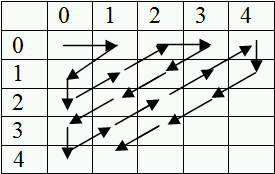
\includegraphics{countablyinfinitepairs.png}


Assume that all different combinations of y run on the horizontal axis and all different values of t runs on the vertical axis. Since for a \textsc{yes} instance x, we know that $M_x$ accepts a y(which contains a 0 at some position) in finite steps, we know that if we can enumerate all possible pairs of (y,t), we will eventually find that particular y and the machine $M_x$ would accept. The reason for choosing the values of t and v in such a manner would ensure we cover all possible combinations of these pairs. In other words we can number these pairs in a definite manner which would allow us to cover all of them (This set of pairs is a infinitely countable set).\\\\
So we have shown that there exists a turning machine $U$ which would accept all \textsc{yes} strings which satisfy this property, and hence this property is semi decidable and not decidable (proved above).


\end{document}
